\chapter{Практические задания}

\section*{Задание 1. Чем принципиально отличаются функции cons, list, append? Пусть (setf lst1 '( a b c))  и (setf lst2 '( d e)). Каковы результаты вычисления следующих выражений?}

\begin{lstinputlisting}[
	caption={Задание 1},
	label={lst:t1},
	style={lsp},
	linerange={1-6},
	]{../src/main.lsp}
\end{lstinputlisting}

\section*{Задание 2. Каковы   результаты   вычисления   следующих   выражений,   и   почему?}

\begin{lstinputlisting}[
	caption={Задание 2},
	label={lst:t2},
	style={lsp},
	linerange={8-17},
	]{../src/main.lsp}
\end{lstinputlisting}

\section*{Задание 3.  Написать, по крайней мере, два варианта функции, которая возвращает последний элемент своего списка-аргумента.}

\begin{lstinputlisting}[
	caption={Задание 3, вариант 1},
	label={lst:t3-1},
	style={lsp},
	linerange={27-39},
	]{../src/main.lsp}
\end{lstinputlisting}

\begin{lstinputlisting}[
	caption={Задание 3, вариант 2},
	label={lst:t3-2},
	style={lsp},
	linerange={23-25},
	]{../src/main.lsp}
\end{lstinputlisting}

\begin{lstinputlisting}[
	caption={Задание 3, вариант 3},
	label={lst:t3-3},
	style={lsp},
	linerange={19-21},
	]{../src/main.lsp}
\end{lstinputlisting}


\section*{Задание 4. Написать, по крайней мере, два варианта функции, которая возвращает свой список аргумент без последнего элемента. }

\clearpage

\begin{lstinputlisting}[
	caption={Задание 4, вариант 1},
	label={lst:t4-1},
	style={lsp},
	linerange={41-53},
	]{../src/main.lsp}
\end{lstinputlisting}

\begin{lstinputlisting}[
	caption={Задание 4, вариант 2},
	label={lst:t4-2},
	style={lsp},
	linerange={55-57},
	]{../src/main.lsp}
\end{lstinputlisting}

\section*{Задание 5. Напишите   функцию   swap-first-last,   которая   переставляет   в   списке-аргументе первый и последний элементы.}

\begin{lstinputlisting}[
	caption={Задание 5},
	label={lst:t5},
	style={lsp},
	linerange={59-66},
	]{../src/main.lsp}
\end{lstinputlisting}

\section*{Задание 6. }
Написать простой вариант игры в кости, в котором бросаются две правильные кости. Если сумма выпавших очков равна 7 или 11   — выигрыш, если выпало (1,1) или (6,6)   — игрок имеет право снова бросить кости, во всех остальных случаях ход переходит ко второму игроку, но запоминается сумма выпавших очков. Если второй игрок не выигрывает абсолютно, то выигрывает тот игрок, у которого больше очков. Результат игры и значения выпавших костей выводить на экран с помощью функции print.

\begin{lstinputlisting}[
	caption={Задание 6},
	label={lst:t6},
	style={lsp},
	linerange={67-127},
	]{../src/main.lsp}
\end{lstinputlisting}

\section*{Задание 7. Написать функцию, которая по своему списку-аргументу lst определяет является ли он палиндромом (то есть равны ли lst и (reverse lst)).}

\begin{lstinputlisting}[
	caption={Задание 7},
	label={lst:t7},
	style={lsp},
	linerange={145-147},
	]{../src/main.lsp}
\end{lstinputlisting}

\section*{Задание 8. Напишите свои необходимые функции, которые обрабатывают таблицу из 4-х точечных пар: (страна . столица), и возвращают по стране - столицу, а по столице — страну.}

\begin{lstinputlisting}[
	caption={Задание 8, IF},
	label={lst:t8},
	style={lsp},
	linerange={149-155},
	]{../src/main.lsp}
\end{lstinputlisting}

\section*{Задание 9.}
Напишите функцию, которая умножает на заданное число-аргумент 
первый числовой элемент списка из заданного 3-х элементного списка-
аргумента, когда

a) все элементы списка --- числа,

6) элементы списка -- любые объекты.


\begin{lstinputlisting}[
	caption={Задание 9, a},
	label={lst:t9-1},
	style={lsp},
	linerange={157-171},
	]{../src/main.lsp}
\end{lstinputlisting}

\begin{lstinputlisting}[
	caption={Задание 9, b},
	label={lst:t9-1},
	style={lsp},
	linerange={173-179},
	]{../src/main.lsp}
\end{lstinputlisting}


%\begin{figure}[h!]
%	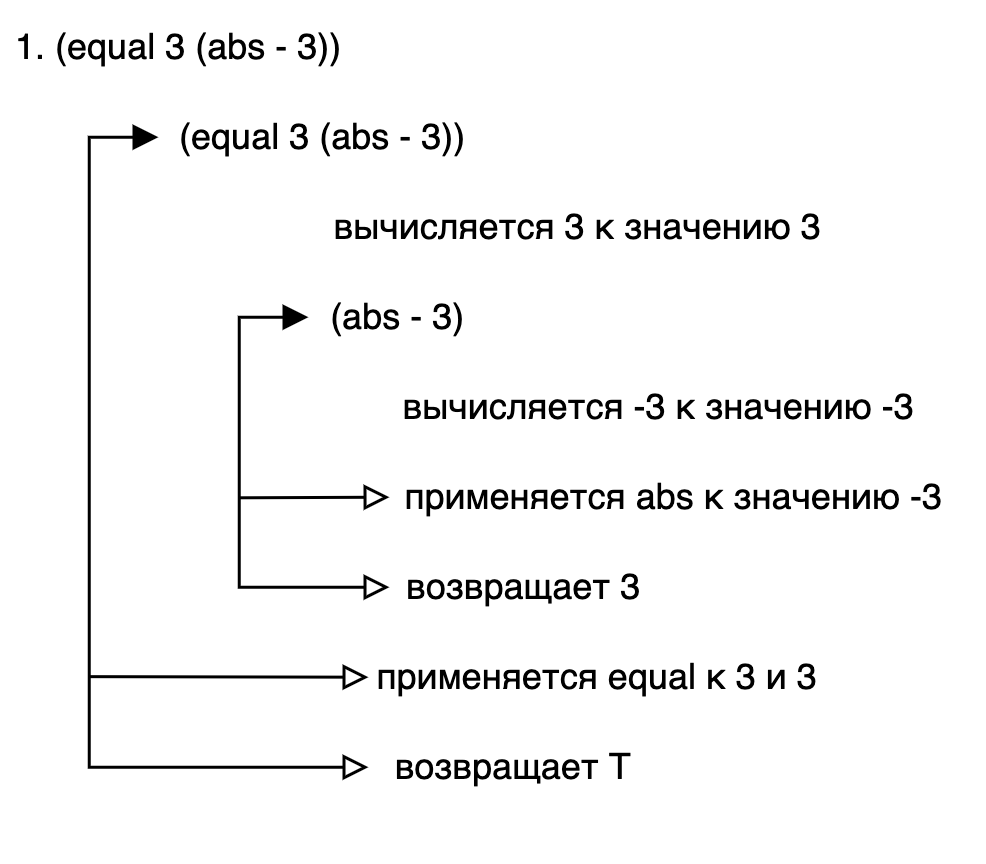
\includegraphics[scale=0.6,left]{task1.1}
%\end{figure}



